
\documentclass{beamer}
\usepackage{tcolorbox}
\usepackage{caption}
\usepackage{pgfplots}
\usepackage{pdfpages}
\usepackage{grffile}
%\beamerdefaultoverlayspecification{<+->}
\newcommand{\data}{\mathcal{D}}

\DeclareMathOperator*{\argmin}{arg\,min}

\newcommand\Item[1][]{%
	\ifx\relax#1\relax  \item \else \item[#1] \fi
	\abovedisplayskip=0pt\abovedisplayshortskip=0pt~\vspace*{-\baselineskip}}


\usetheme{metropolis}           % Use metropolis theme


\title{Lasso Regression}
\date{\today}
\author{Nipun Batra}
\institute{IIT Gandhinagar}
\begin{document}
  \maketitle
  
  
  
  
% \section{Linear Regression}

\begin{frame}{Lasso Regression}
\begin{itemize}[<+->]
	
	
	\item LASSO $\longrightarrow$ Least absolute shrinkage and selection operator
	\item Popular as it leads to a sparse solution.
	
\end{itemize}
\end{frame}

\begin{frame}{Constructing the Objective Function}
\begin{itemize}[<+->]

\item Find a $\theta_{opt}$ such that  \begin{equation}    \theta_{opt} =  \argmin_{\theta} {(Y-X\theta)^T(Y-X\theta)} : \ |\theta|<s \end{equation}
\item Using KKT conditions
\begin{equation}
    \theta_{opt} = \underbrace{\argmin_{\theta}{(Y-X\theta)^T(Y-X\theta) + \delta^2|\theta|}}_\text{convex function}
\end{equation}
	
\end{itemize}


\end{frame}

\begin{frame}{Solving the Objective}
\begin{itemize}[<+->]

\item Since $|\theta|$ is not differentiable, we cannot solve,  \begin{equation}    \frac{\partial {(Y-X\theta)^T(Y-X\theta) + \delta^2|\theta|}}{\partial \theta} = 0 \end{equation}

\item How to Solve?
Use Coordinate descent!
\end{itemize}

\end{frame}

\begin{frame}{Sample Dataset}

\begin{figure}
    \centering
    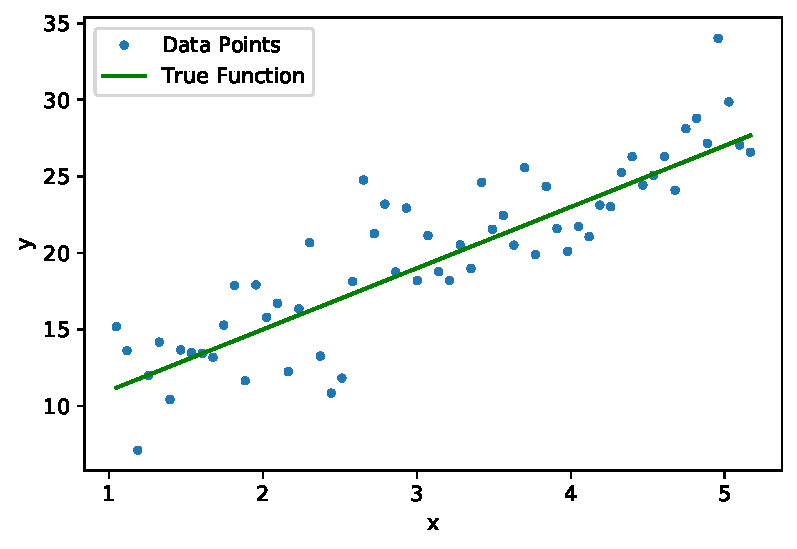
\includegraphics[scale = 0.75]{Lasso/true_function.pdf}
    \caption{y = 4x + 7}
    \label{fig:my_label}
\end{figure}{}

\end{frame}

\begin{frame}{Geometric Interpretation}
\begin{figure}
    \centering
    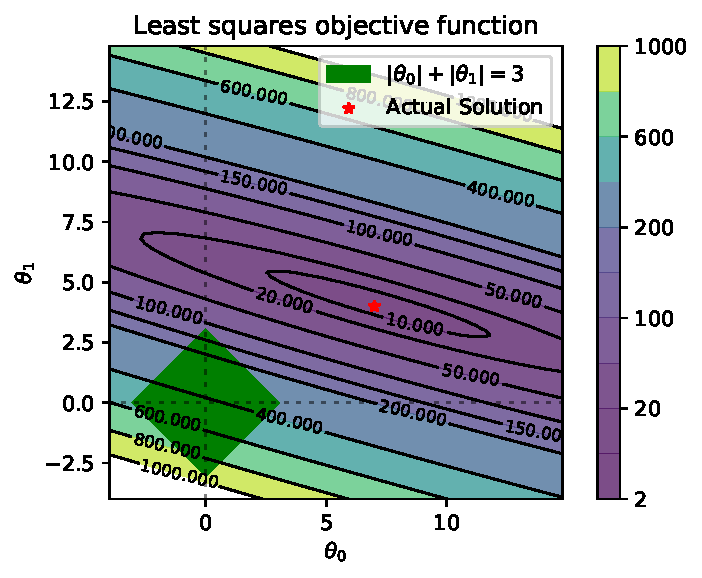
\includegraphics[scale = 0.75]{Lasso/lasso_base_contour.pdf}
    \caption{Lasso regression}
    \label{fig:my_label}
\end{figure}

\end{frame}

\begin{frame}{Effect of $\mu$ - Regularization of Parameters}
\vspace{0.4cm}
\begin{figure}

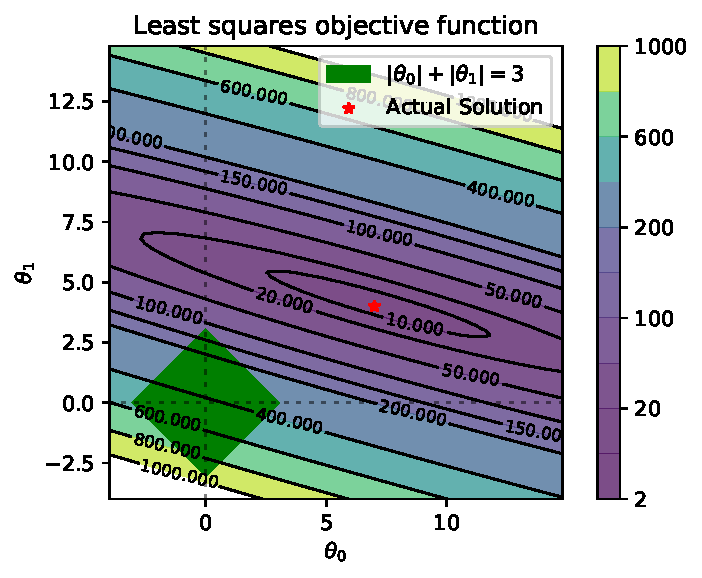
\includegraphics[width=0.9\linewidth]{Lasso/lasso_base_contour.pdf}
\caption{$\mu = 1.0$\\(on the \emph{Sample Dataset})}
\end{figure}
\end{frame}

\begin{frame}{Effect of $\mu$ - Regularization of Parameters}
\vspace{0.4cm}
\begin{figure}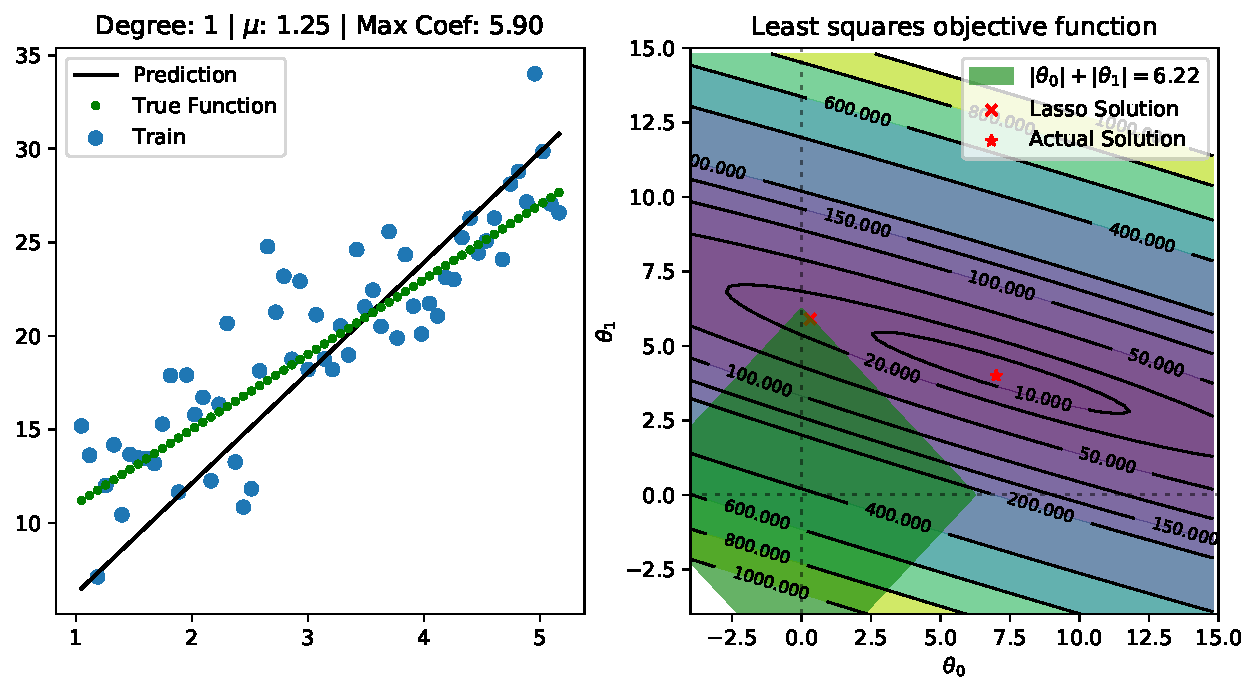
\includegraphics[width=0.9\linewidth]{Lasso/lasso_1.25.pdf}\caption{$\mu = 1.25$\\(on the \emph{Sample Dataset})}
\end{figure}
\end{frame}

\begin{frame}{Effect of $\mu$ - Regularization of Parameters}
\vspace{0.4cm}
\begin{figure}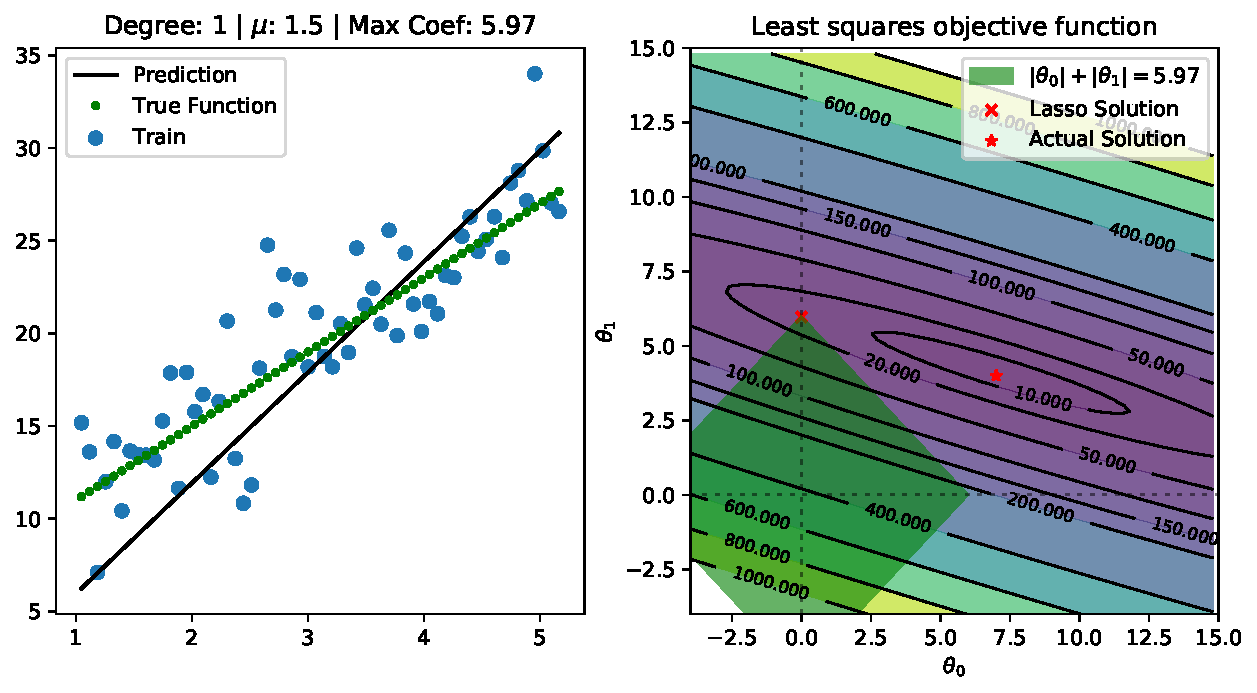
\includegraphics[width=0.9\linewidth]{Lasso/lasso_1.5.pdf}\caption{$\mu = 1.5$\\(on the \emph{Sample Dataset})}
\end{figure}
\end{frame}

\begin{frame}{Effect of $\mu$ - Regularization of Parameters}
\vspace{0.4cm}
\begin{figure}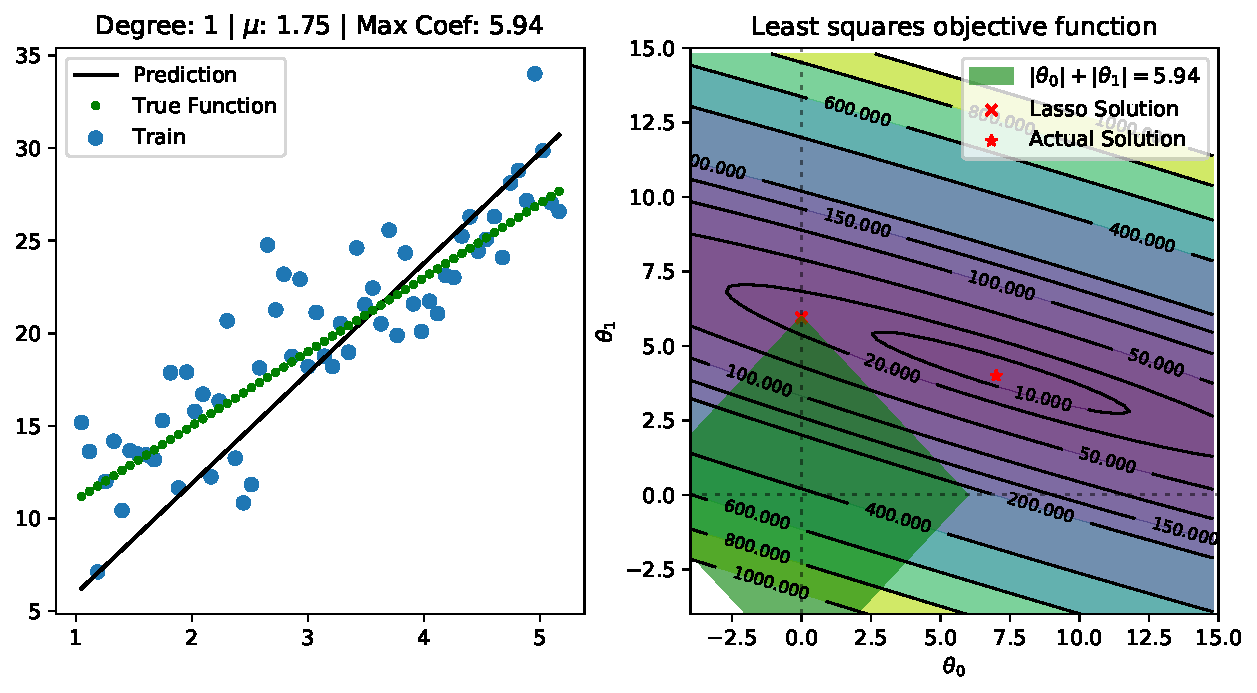
\includegraphics[width=0.9\linewidth]{Lasso/lasso_1.75.pdf}\caption{$\mu = 1.75$\\(on the \emph{Sample Dataset})}
\end{figure}
\end{frame}


\begin{frame}{Effect of $\mu$ - Regularization of Parameters}
\vspace{0.4cm}
\begin{figure}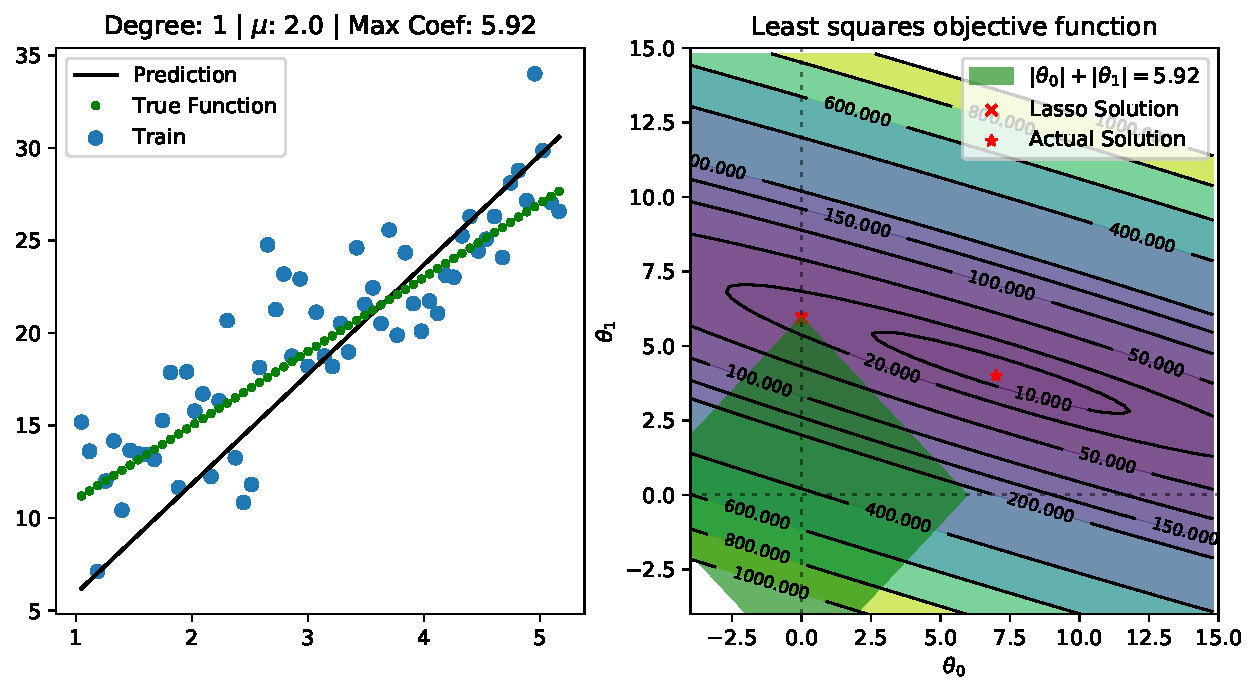
\includegraphics[width=0.9\linewidth]{Lasso/lasso_2.0.pdf}\caption{$\mu = 2.0$\\(on the \emph{Sample Dataset})}
\end{figure}
\end{frame}

{
	\setbeamercolor{background canvas}{bg=}
	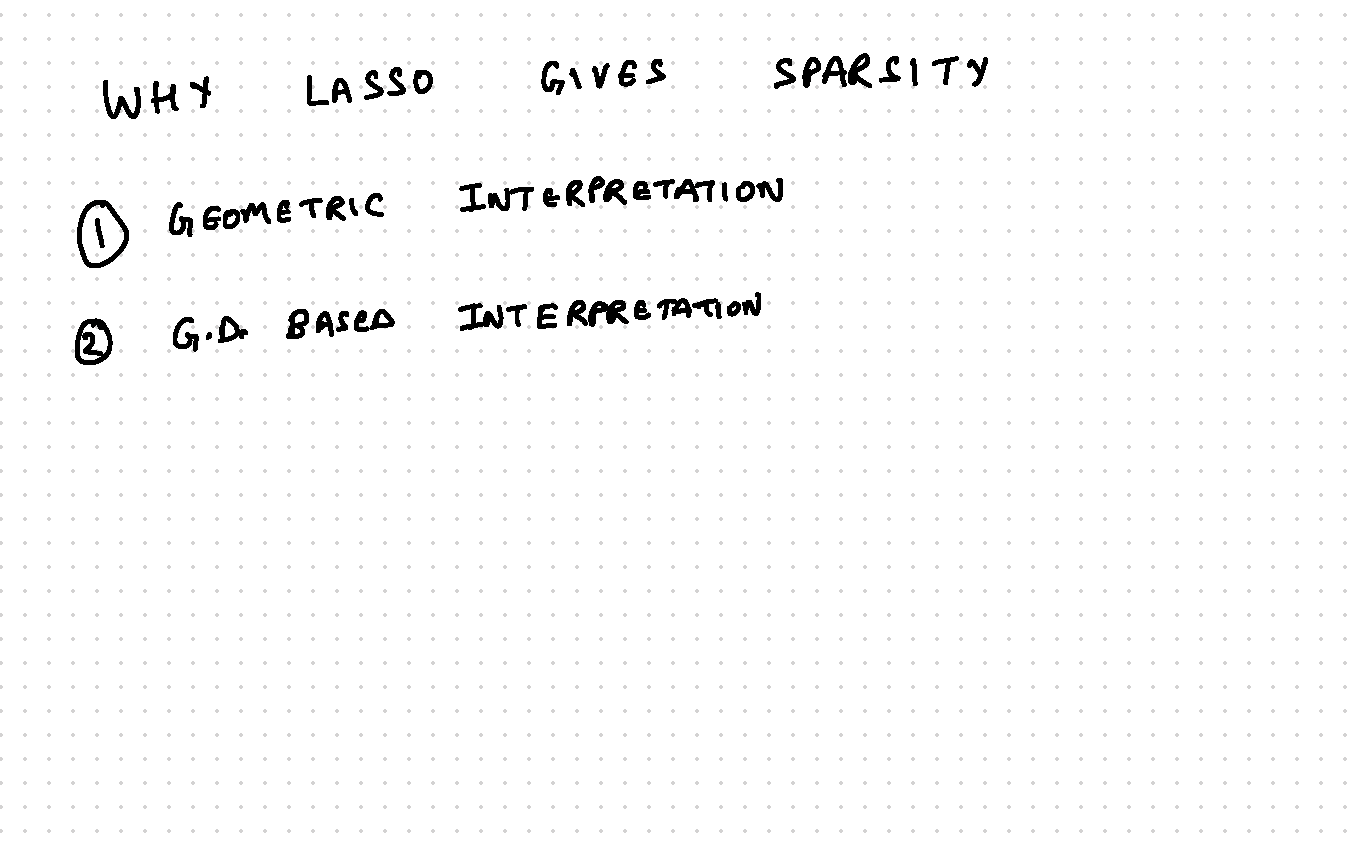
\includepdf[page=-]{lasso-sparse.pdf}
}


%\begin{frame}{Why Lasso Gives Sparse solution}
%\begin{figure}
%    \centering
%    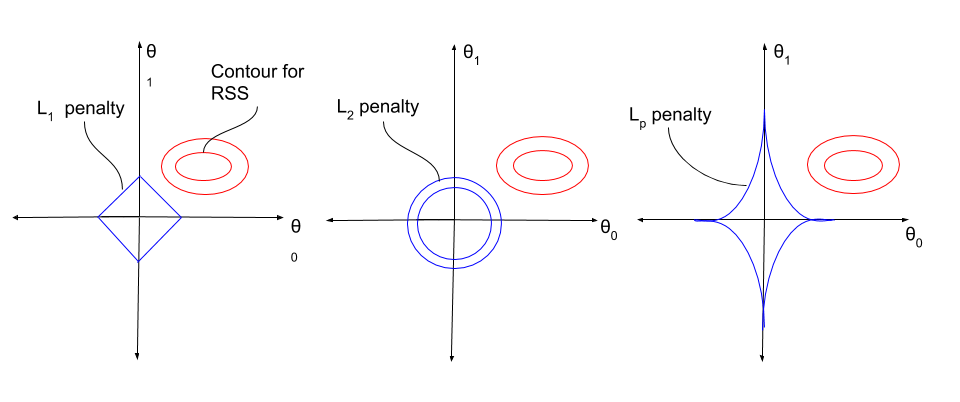
\includegraphics[scale = 0.4]{Lasso/lasso_2.png}
%    \label{fig:my_label}
%\end{figure}
%\begin{itemize}
%\small{
%    \item Pointedness of $L_{p}$ norm 
%    \item  Probability of Intersecting an axis increases.
%    \item Sparsity increases. 
%    \item Solving difficulty also increases
%    }
%\end{itemize}
%
%\end{frame}
%
%\begin{frame}{Interpretation : II}
%\begin{figure}
%    \centering
%    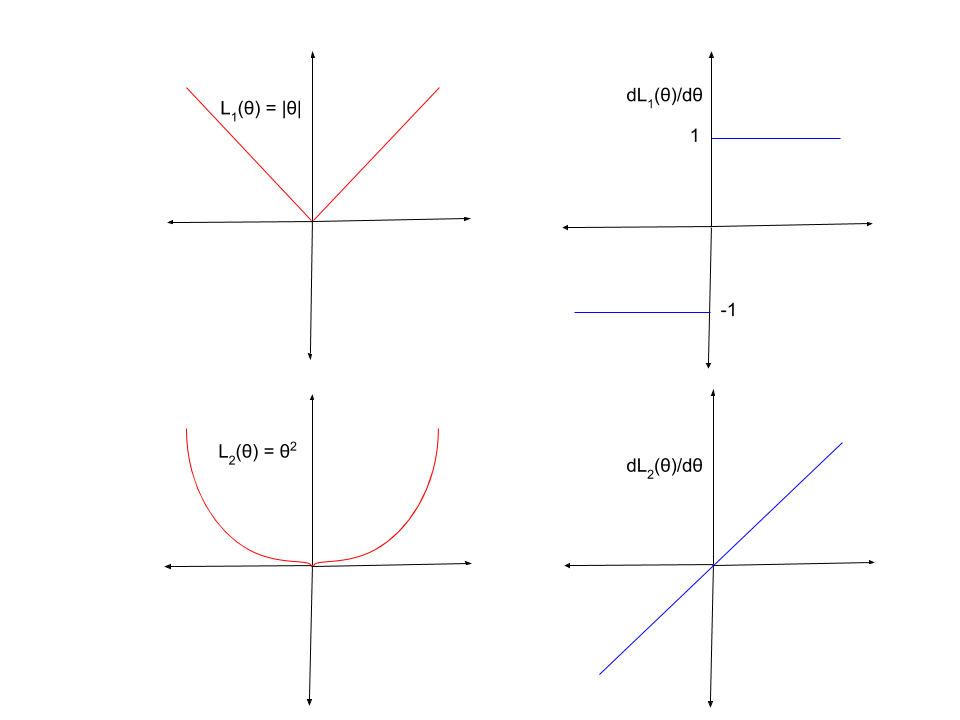
\includegraphics[scale = 0.3]{Lasso/lasso_3.png}
%    \label{fig:my_label}
%\end{figure}
%
%\end{frame}
%
%
%
%\begin{frame}{Gradient Descent}
%
%
%\foreach \x in {0,1,2,3,4} 
%{%
%\includegraphics<\x>[scale=0.75]{Lasso/GD_iteration_\x.pdf}
%%    
%}
%
%
%\end{frame}

\begin{frame}{Regularization path of lasso regression}
\begin{figure}
    \centering
    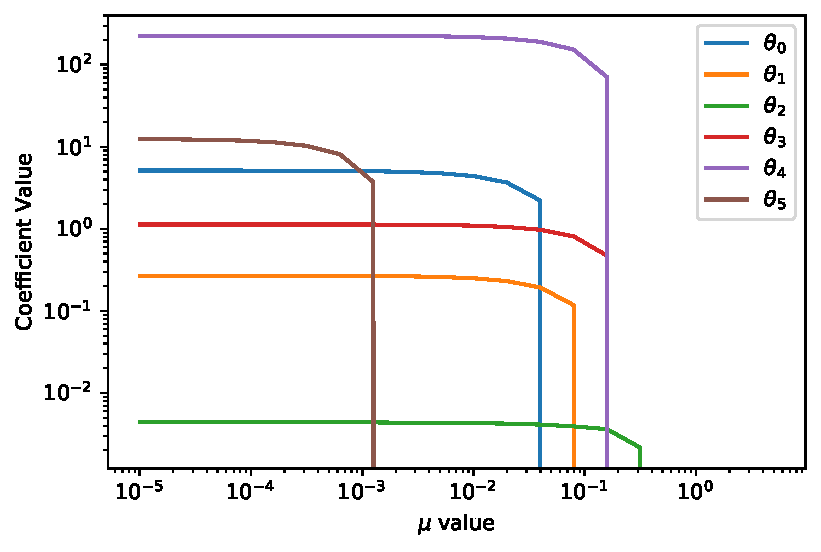
\includegraphics[scale = 0.5]{Lasso/lasso_reg.pdf}
    \caption{Regularization path of $\theta_{i}$}
    \label{fig:my_label}
\end{figure}

\end{frame}



\end{document}